\documentclass[12pt]{article}

\usepackage{sbc-template}

\usepackage{graphicx,url}

\usepackage[brazil]{babel}
%\usepackage[latin1]{inputenc}
\usepackage[utf8]{inputenc}


\sloppy

\title{Implementando o \textit{Marching Squares} em HTML5 e JavaScript para navegadores}

\author{Vinicius Junqueira Schettino\inst{1}}


\address{Departamento de Ciência da Computação (DCC) --- Universidade Federal de Juiz\\de Fora (UFJF)
\email{vinicius.schettino@ice.ufjf.br}
}

\begin{document}

\maketitle

\begin{resumo}
  Aplicações \textit{web} apresentam cada vez mais funcionalidades e interatividade com seus utilizadores. Tal advento está diretamente relacionado à crescente capacidade computacional dos navegadores, que cada vez mais executam tarefas complexas sem grande interferência do servidor para apoiar a experiência do usuário e a distribuição do processamento. Assim, este trabalho propõe a implementação da extração de contornos de figuras utilizando HTML5 e JavaScript, buscando apoiar funcionalidades de reconhecimento e processamento de imagens \textit{client-side} com tecnologias modernas e preparadas para a nova geração de aplicações. Através do algoritmo \textit{marching squares}, o contorno é encontrado e demonstrado para o usuário. Um benchmark simples ajuda a avaliar o algoritmo e futuras otimizações da codificação.
\end{resumo}


\section{Introdução}

O \textit{marching squares} é um algoritmo de detecção de contorno para matrizes bidimensionais,
\section{Métodos e Ferramentas}\label{sec:firstpage}. Pode ser utilizado para inúmeras funcionalidades dentro do processamento de imagens, notalvemente para reconhecimento de padrões e seleção e extração de subconjuntos~\cite{hanisch2004}. A técnica também pode ser extendida para atuar sobre campos tridimensionais de maneira muito próxima ao funcionamento original~\cite{maple2003}.

Através da implementação proposta neste trabalho, é possível desenvolver funcionalidades que dependam apenas do navegador, sem consumir recursos de rede ou processamento do servidor. Esta característica pode ser útil para aplicações de tempo real como interfaces de edição de imagens ou de reconhecimento, como jogos ou utilitários simples.

\section{implementação}

Através do trabalho de~\cite{spiess2010}, observou-se o funcionamento do algoritmo e adatapções necessárias para funcionamento com JavaScript. Outras implementações também foram consultadas\footnote{https://gist.github.com/mieko/3c17c41b8be9f2598c12} para melhor entendimento do algoritmo e separar estes conceitos das limitações de cada linguagem.

A implementação do \textit{marching squares} foi encapsulada em uma classe (no conceito JavaScript) separada em um arquivo específico. Os métodos deste componente foram utilizados através de um script dentro da página principal do algoritmo. O resultado pode ser visto na figura~\ref{fig:marching}.

Para estilização da aplicação foi utilizado o Boostrap v4.0.0-aplha.6\footnote{https://v4-alpha.getbootstrap.com/}. Através de um contador simples de tempo, infere-se e apresenta-se o tempo necessário para execução do algoritmo.
\begin{figure}[ht]
\centering
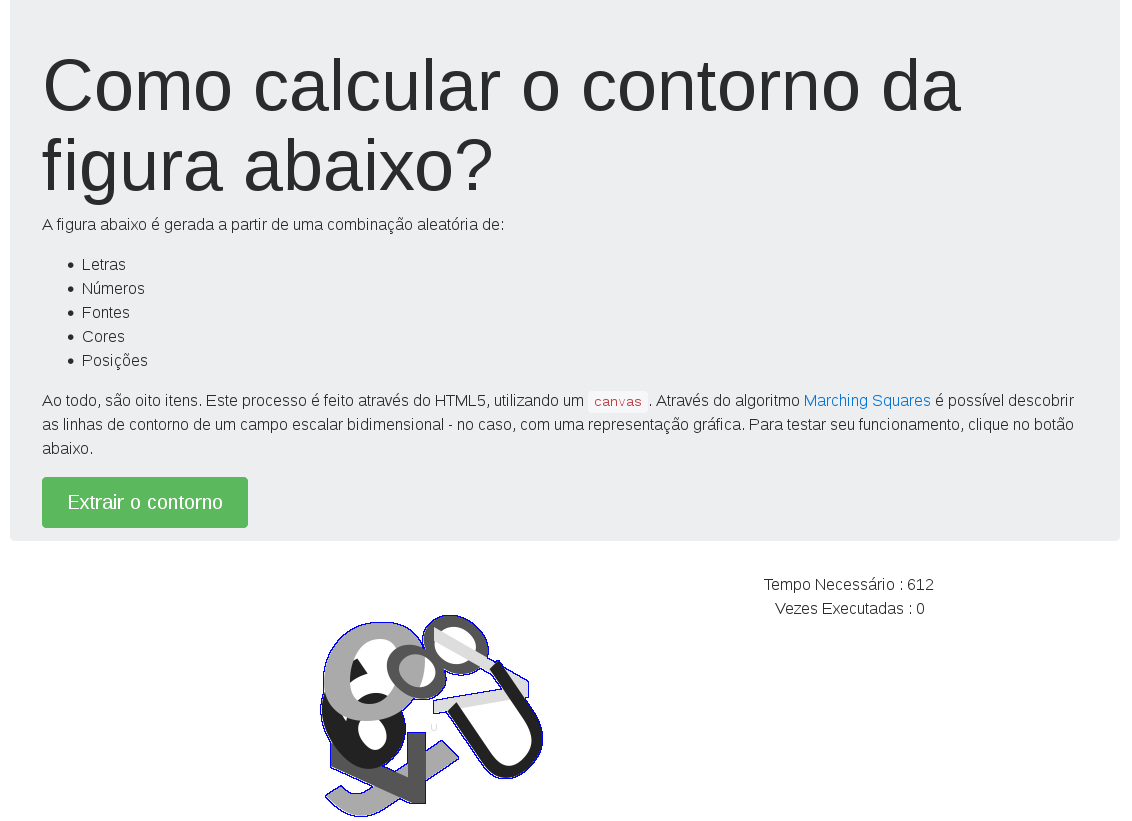
\includegraphics[width=\textwidth]{marching.png}
\caption{Funcionamento do algoritmo. O contorno azul da figura foi gerado pelo \textit{marching squares}}
\label{fig:marching}
\end{figure}

\section{considerações finais}

O \textit{marching squares} pode ser utilizado para diversas aplicações no âmbito de processamento de imagens, em particular na detecção e extração de padrões. Através deste trabalho apresenta-se uma implementação de tal técnica voltada para uso \textit{client-side} em aplicações para internet, onde todo o processamento é realizado com recursos computacionais disponíveis pelo navegador.

A utilização de tecnologias modernas como o HTML5 e o JavaScript permitem a incorporação desta implementação em aplicações atuais e igualmente modernas, prepando-as para a nova geração de utilizadores e requisitos, funcionais e não funcionais.

Como trabalhos futuros, pretendemos avaliar o desempenho da implementação aqui descrita em comparação com outros métodos, levando em consideração particularidades da linguagem e do contexo ao qual se propõe esta solução.

\bibliographystyle{sbc}
\bibliography{sbc-template}

\end{document}
